\documentclass[11pt]{article}
\usepackage{graphicx}
\usepackage[authoryear,round]{natbib}
\usepackage{caption}
\usepackage{subcaption}
\usepackage[mathlines]{lineno}
\usepackage{setspace}
\usepackage{mathrsfs}
\usepackage{rotating}
\usepackage{url}
\usepackage{amssymb}
\usepackage{multirow}
\usepackage[none]{hyphenat}
\usepackage{algpseudocode}
\DeclareGraphicsExtensions{.pdf,.png,.jpg}
\setlength{\topmargin}{-0.5in}
\setlength{\textheight}{10in}
\setlength{\oddsidemargin}{.125in}
\setlength{\textwidth}{6.25in}
\doublespacing
\pagestyle{empty}

\captionsetup[subfigure]{labelfont=rm}

\begin{document}

\begin{figure}[h!]
\begin{center}
   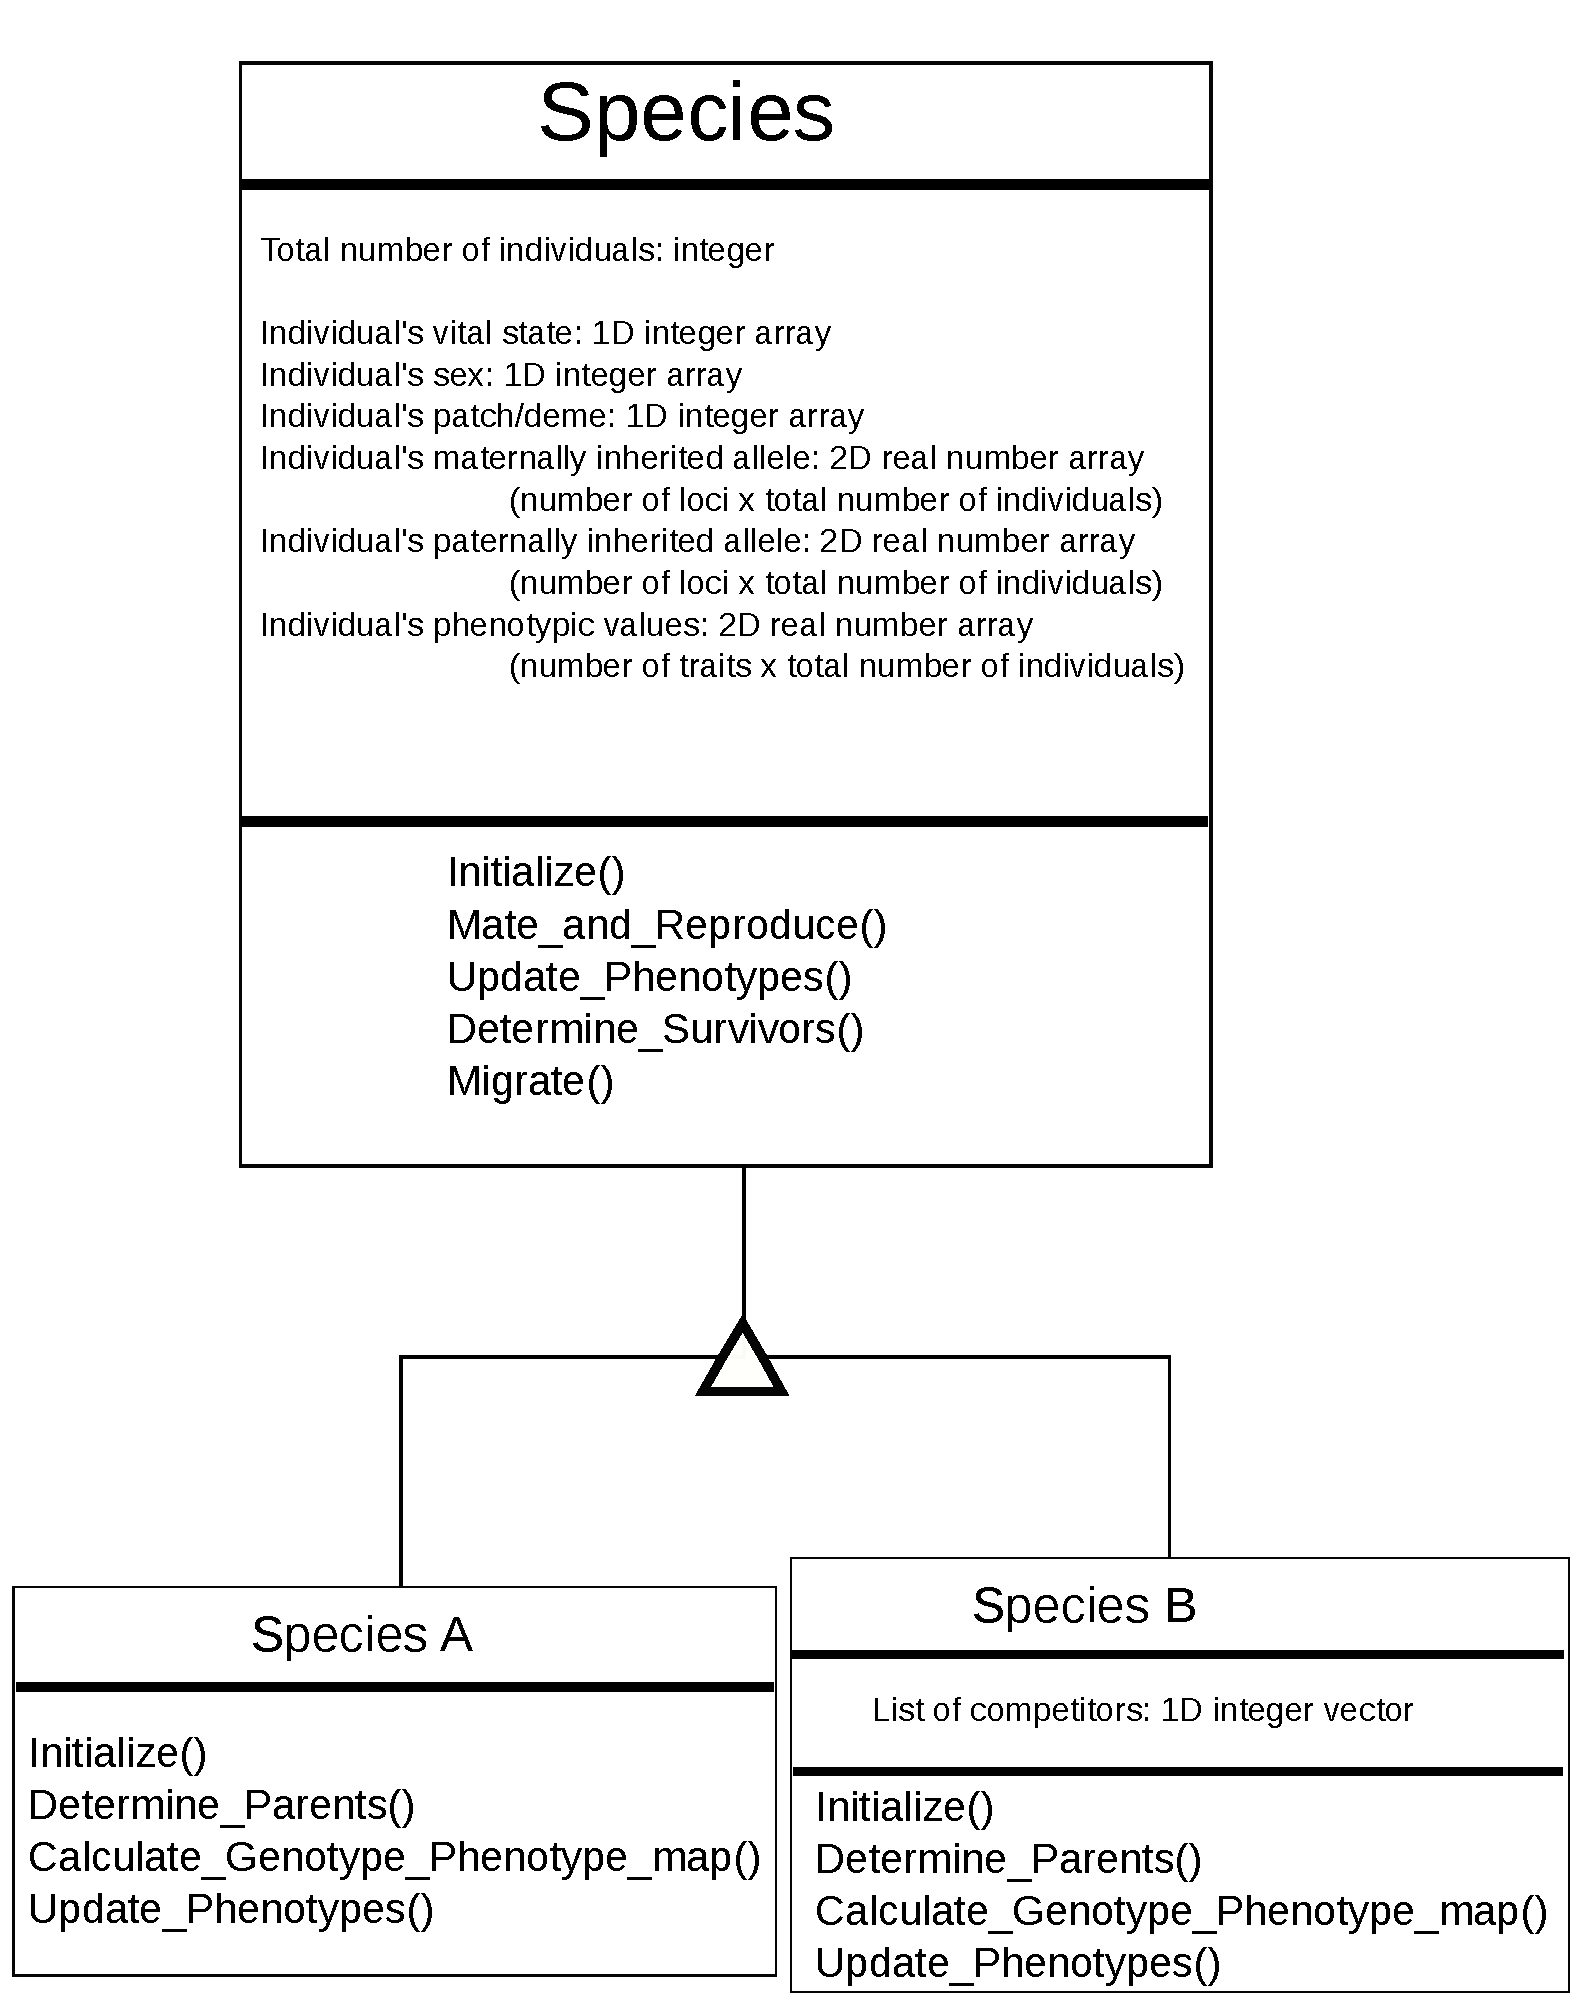
\includegraphics[width=0.9\linewidth] {SupplementaryFigures/FigS4.pdf}
\end{center}
\caption*{Figure S4.  A description of the base class for species that is used in sPEGG, and example relationships to derived, model-specific classes (species A and species B) using the object modelling technique. The first segment of each box speciefies the class name, the middle (if present) segment specifies the data members of the class, and the last segment lists the methods (functions) of the class. In this example, the methods \texttt{Initialize()}, \texttt{Determine\_Parents()}, \texttt{Calculate\_Genotype\_Phenotype\_map()} and \texttt{Update\_Phenotypes()} implement alternative, species-specific customizable routines that can potentially differ between species A and species B (e.g., different genetic architectures), and species B also contains a data member consisting of the indices of potential competitors (e.g., individuals in species A that potentially pre-empt resources from species B). The remaining attributes are common to species A and species B, as are the routines for simulating mating and reproduction, mortality, and migration.}
\end{figure}	
\end{document}

